\subsection{Definition}
This example is presented for code verification of different element types, i.e. lines, triangles, quads, tetrahedra, triangle prisms and hexahedra \cite{WanKol:2007}. We consider a non-linear problem, flow of a compressible fluid through the porous medium. In this case the hydraulic conductivity is pressure dependent.


The discretization with different element types is shown in Fig. \ref{fig:h_elements}. The initial gas pressure distribution is equal to $1.01325\times10^5 \mathrm{Pa}$; everywhere in the model domain. There are Dirichlet boundary condition set at left end, i.e. $p^g(x=0 \mathrm m) = 9.5500\times10^4\mathrm{Pa}$, and right end, i.e. $p^g(x=100 \mathrm m) = 1.01325\times10^5\mathrm{Pa}$, in order to extract gas from the domain. The material parameters of the fluid and the porous medium are given in Tab. \ref{tab:apl_h}.
\begin{figure}[htb!]
\center
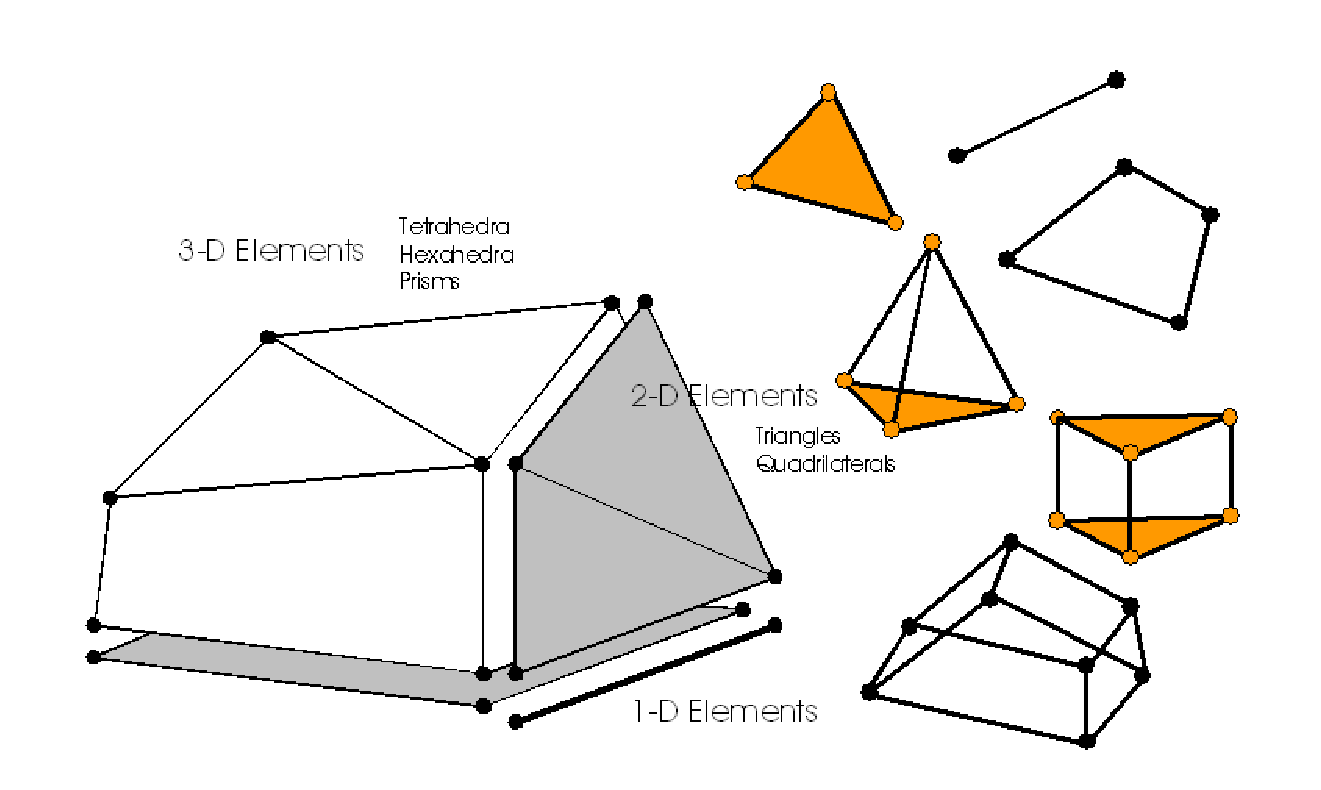
\includegraphics[scale=0.45]{PART_II/G/elements.eps}
\caption{Different element types.} 
\label{fig:h_elements}
\end{figure}
\begin{table}[htb]
\caption{\label{tab:apl_h}Material parameters.}
\begin{center}
\begin{tabular}{llrr}
\toprule
Symbol & Parameter & Value & Unit \\
\midrule
$L$ & Model length & $0.05$ & $\mathrm m$\\
$A$ & Cross section area & $1$  & $\mathrm{m^2}$ \\
$\mu$ & Dynamic viscosity & 1.78$\times 10^{-5}$ & $\mathrm{Pa s}$ \\
$n$ & Porosity & 0.005 & $-$\\
$\k$ & Permeability & 2.77$\times 10^{-19}$ & $\mathrm{m^2}$ \\
$\Delta t$ & Time step & $ 3\times 10^2$ & $\mathrm{s}$\\
$\Delta x$ & Space step & $0.005$ & $\mathrm{m}$\\
\bottomrule
\end{tabular}
\end{center}
\end{table}
\begin{figure}[htb!]
\center
\includegraphics[scale=0.3]{PART_II/G/gas_flow.eps}
\caption{Evolution of gas pressure at the outlet observation point.}
\label{fig:gas_flow}
\end{figure}
\subsection{Results}
Fig. \ref{fig:gas_flow} depicts the temporal evolution of gas pressure at the observation point at the outlet. The numerical results of all implemented element types compare very well. Small deviation occur from different numbers of Gauss integration points.
